\chapter{Testes e Simulações}

Para ilustrar o funcionamento dos algoritmos, foi proposta uma planta hidráulica composta por um sistema de tanques comunicantes. A figura \ref{fig:TanquesComunicantes} mostra um esboço de tal sistema. O tanque com capactância $C_1$ é interligado com um de capacitância $C_2$. Aquele é alimentado por uma vazão $q$ e é drenado por uma vazão $q_1$. Tal grandeza é controlada por um registro, que pode ser enxergado como um resistor de resistência $R_1$.

Ainda, devido à ligação, a vazão de saída do primeiro tanque é a entrada do segundo. Este é drenado por uma vazão $q_2$, onde é controlado por um registro $R_2$. A variável controlada é a diferença $h_1 - h_2$.

\begin{figure}[!ht]
  \centering
  \usetikzlibrary{calc}
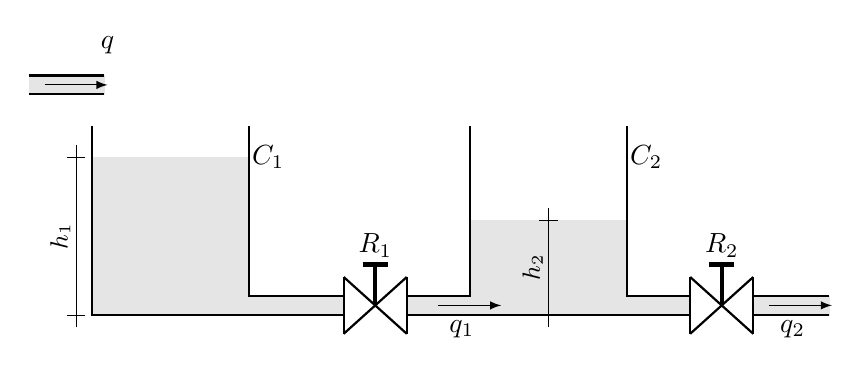
\begin{tikzpicture}[scale=0.8]
    \draw [ultra thin,color=Gray!20,fill] (0,-.5) rectangle (2.5,-3);
    \draw [ultra thin,color=Gray!20,fill] (2.5,-3) rectangle ++(1.5,.3);
    \draw [ultra thin,color=Gray!20,fill] (6,-1.5) rectangle (8.5,-3);
    \draw [ultra thin,color=Gray!20,fill] (10.5,-3) rectangle ++(1.2,.3);
    \draw [thick] (0,0) -- (0,-3) -- ++(4,0) coordinate(FimDoCano);
    \draw [thick] ($(FimDoCano)+(0,.3)$) -- ++(-1.5,0) -- ++(0,2.7);
    
    \draw [ultra thin,color=Gray!20,fill] ($(FimDoCano)+(1,0)$) rectangle ++(4.5,.3);
    \draw [thick] ($(FimDoCano)+(0,-.3)$) -- ++(0,.9);
    \draw [thick] ($(FimDoCano)+(0,-.3)$) -- ++(1,.9);
    \draw [thick] ($(FimDoCano)+(1,.6)$) -- ++(0,-.9);
    \draw [thick] ($(FimDoCano)+(1,-.3)$) -- ($(FimDoCano)+(0,.6)$);
    \draw [ultra thick] ($(FimDoCano)+(.5,.15)$) -- ++(0,.65) coordinate (Registro);
    \draw [ultra thick] ($(Registro)+(-.2,0)$) -- ($(Registro)+(.2,0)$);
    \draw [-latex] ($(FimDoCano)+(1.5,.15)$) -- ++(1,0) node [xshift=-.5cm,yshift=-.3cm] {$q_1$};
    \draw [thick] ($(FimDoCano)+(1,0)$) -- ++(4.5,0) ++(0,.3) -- ++(-1,0) -- ++(0,2.7) ++(-2.5,0) -- ++(0,-2.7) -- ++(-1,0);
    \draw [thick] ($(FimDoCano)+(5.5,-.3)$) -- ++(0,.9);
    \draw [thick] ($(FimDoCano)+(5.5,-.3)$) -- ++(1,.9);
    \draw [thick] ($(FimDoCano)+(6.5,.6)$) -- ++(0,-.9);
    \draw [thick] ($(FimDoCano)+(6.5,-.3)$) -- ($(FimDoCano)+(5.5,.6)$);
    \draw [ultra thick] ($(FimDoCano)+(6,.15)$) -- ++(0,.65) coordinate (Registro2);
    \draw [ultra thick] ($(Registro2)+(-.2,0)$) -- ($(Registro2)+(.2,0)$);\draw [very thin] (-.1,-3) -- ++(-.3,0);
    \draw [very thin] (-.1,-.5) -- ++(-.3,0);
    \draw [very thin] (-.25,-3.2) -- ++(0,2.9);
    \node [rotate=90] at (-.5,-1.75) {\small$h_1$};
    \draw [very thin] (7.4,-1.5) -- ++(-.3,0);
    \draw [very thin] (7.25,-3.2) -- ++(0,1.9);
    \node [rotate=90] at (7,-2.25) {\small$h_2$};
    \node (NomedoRegistro) at ($(Registro)+(0,.3)$) {$R_1$};
    \node (NomedoTanque) at ($(FimDoCano)+(-1.2,2.5)$) {$C_1$};
    \node (NomedoRegistro2) at ($(Registro2)+(0,.3)$) {$R_2$};
    \node (NomedoTanque2) at ($(FimDoCano)+(4.8,2.5)$) {$C_2$};
    \draw [ultra thin,color=Gray!20,fill] (-1,.5) rectangle ++(1.2,.3);
    \draw [thick] (-1,.5) -- ++(1.2,0) ++(0,.3) -- ++(-1.2,0);
    \draw [-latex] (-.75,.65) -- ++(1,0) node [yshift=.5cm] {$q$};
    \draw [thick] (10.5,-3) -- ++(1.2,0) ++(0,.3) -- ++(-1.2,0);
    \draw [-latex] (10.75,-2.85) -- ++(1,0) node [xshift=-.5cm,yshift=-.3cm] {$q_2$};
\end{tikzpicture}
  \caption{Tanques comunicantes.}
  \label{fig:TanquesComunicantes}
\end{figure}

\section{Modelagem via espaço de estados}
Para a representação via espaço de estados, define-se as variáveis de estado $x_1 = q_1$ e $x_2 = q_2$. A partir das relações entre capacitância e vazão, chega-se a seguinte representação no espaço de estados:
\begin{subequations}
  \begin{align}
    \dot{\pmb{\mathrm{x}}} &= \begin{bmatrix*}[c]
      -(R_1C_{eq})^{-1} & (R_1C_2)^{-1}\\
      (R_2C_2)^{-1} & -(R_2C_2)^{-1}
    \end{bmatrix*}\pmb{\mathrm{x}} + \begin{bmatrix*}[c]
      (R_1C_1)^{-1}\\
      0
    \end{bmatrix*}\mathrm{u}\label{eq:SSEntrada}\\
    \mathrm{y} &= \begin{bmatrix*}[c]
      R_1 & 0
    \end{bmatrix*}\pmb{\mathrm{x}}\label{eq:SSSaida}
  \end{align}
\end{subequations}
onde $C_{eq} = C_1C_2/(C_1 + C_2)$. Para discretizar o sistema, é preciso de um valor para o período de amostragem $T_s$. A transformada usada será a bilinear de Tustin, dada por:
\begin{equation}
  \s = \dfrac{2}{T_s}\dfrac{\z-1}{\z+1}\label{eq:BilinearTransform}
\end{equation}
onde o semi-plano esquerdo dos contínuos é mapeado no círculo unitário dos discretos.

\section{Primeiro projeto}
Com posse do espaço de estados, é possível sintetizar uma matriz de ganho $K$ que possa estabilizar o sistema. Antes, é necessário atribuir valores para a planta. Em um primeiro projeto, serão escolhidas arbitrariamente tais valores, como segue:
\begin{itemize}
  \item $C_1 = C_2 = 5$;
  \item $R_1 = R_2 = 1$;
  \item $T_s = \SI{1.9}{\second}$.
\end{itemize}

Assim, a representação via espaço de estados da planta nos contínuos é:
\begin{subequations}
  \begin{align}
    \dot{\pmb{\mathrm{x}}} &= \begin{bmatrix*}[c]
      -0.4 & -0.2\\
      0.2 & -0.2
    \end{bmatrix*}\pmb{\mathrm{x}} + \begin{bmatrix*}[c]
      0.2\\
      0
    \end{bmatrix*}\mathrm{u}\label{eq:SSCEntrada}\\
    \mathrm{y} &= \begin{bmatrix*}[c]
      1 & 0
    \end{bmatrix*}\pmb{\mathrm{x}}\label{eq:SSCSaida}
  \end{align}
\end{subequations}

Através do função \texttt{c2d} disponibilizada no MATLAB, a transformação bilinear é realizada, resultando em:
\begin{subequations}
  \begin{align}
    \dot{\pmb{\mathrm{x}}} &= \begin{bmatrix*}[c]
      -0.4181 & -0.2264\\
      0.2264 & -0.6445
    \end{bmatrix*}\pmb{\mathrm{x}} + \begin{bmatrix*}[c]
      0.2694\\
      0.0430
    \end{bmatrix*}\mathrm{u}\label{eq:SSDEntrada}\\
    \mathrm{y} &= \begin{bmatrix*}[c]
      0.7091 & -0.1132
    \end{bmatrix*}\pmb{\mathrm{x}} + \begin{bmatrix*}[c]
      0.1347
    \end{bmatrix*}\mathrm{u}\label{eq:SSDSaida}
  \end{align}
\end{subequations}

A característica notória obtida é a presença da matriz $D$ no sistema discretizado. É um consequência da transformação bilinear: surgimento de transmissão direta. Com posse das matrizes obtidas na representação via espaço de estados, é possível escolher os parâmetros de projeto a serem estudados:
\begin{itemize}
  \item $\zeta = 0.6$;
  \item $\omega_n = \SI{0.5}{\radian/\second}$.
\end{itemize}

Neste caso, a constante $N_y$ possui o valor de $6.6139$, acima do recomendado. Além disso, a maior frequencia natural não amortecida de malha aberta do sistema discretizado possui o valor igual a

\section{Um projeto mais restritivo}
Para exemplificar um projeto mais restritivo, será considerado uma planta com as seguintes características:
\begin{itemize}
  \item $C_1 = 10$;
  \item $C_2 = 10$;
  \item $R_1 = 4$;
  \item $R_2 = 2$;
  \item $T_s = \SI{5}{\second}$.
\end{itemize}

Os parâmetros de projeto são:
\begin{itemize}
  \item $t_s = \SI{30}{s}$;
  \item $M_p = 10\%$;
\end{itemize}

\begin{itemize}
  \item $\sigma = -4/300$;
  \item $\zeta = 0.7$;
  \item $T_s = \SI{5}{\second}$;
  \item $\omega_n = \SI{0.2}{\radian/\second}$.
\end{itemize}